\documentclass[10pt,twocolumn]{article}

% This draft is intentionally venue-neutral. Replace the document class and
% margins with the target conference template once the venue is selected.
% Adult companion paper. Result freeze: 2026-09-11 for local values.
% Biltir values are single-checkpoint and are labelled as such in every table.
% Update on the Biltir server: replace the marked numbers, then rerun.
% Audited local sources: 4 sep presentation.md, ABLATION.md,
% bch-arc-ct/docs/RETRIEVAL_RESULTS_2026-09-07.md, and metric JSON artifacts.
% The later Biltir handoff should be merged only after matching each value to
% its checkpoint, split, input availability, and inference readout.
\usepackage[margin=0.68in,columnsep=0.22in]{geometry}
\usepackage[T1]{fontenc}
\usepackage{lmodern}
\usepackage{microtype}
\usepackage{booktabs}
\usepackage{multirow}
\usepackage{makecell}
\usepackage{tabularx}
\usepackage{threeparttable}
\usepackage{amsmath,amssymb}
\usepackage{graphicx}
\usepackage{xcolor}
\usepackage{tikz}
\usetikzlibrary{arrows.meta,positioning,fit,backgrounds}
\usepackage{pgfplots}
\pgfplotsset{compat=1.18}
\usepackage{hyperref}
\usepackage[capitalize,noabbrev]{cleveref}
\usepackage{enumitem}
\setlist{nosep,leftmargin=*}

\definecolor{ctblue}{HTML}{3977B7}
\definecolor{ctxorange}{HTML}{E68A2E}
\definecolor{ctxgreen}{HTML}{2A9D6F}
\definecolor{lightgray}{HTML}{F2F3F5}
\newcommand{\ours}{\textsc{MetaQ-CT}}
\newcommand{\todo}[1]{\textcolor{red}{[TODO: #1]}}
\newcommand{\best}[1]{\textbf{#1}}


\title{Clinical Metadata-Conditioned Query Formers for\\
Adult Chest CT: How Much Does the Indication Carry?}
\author{Anonymous Authors}
\date{}

\begin{document}
\maketitle

\begin{abstract}
Vision--language models for volumetric chest CT read a scan with generic
pathology prompts. The clinical indication, the patient's age, and the
patient's sex are available at interpretation time and are ignored. We ask
what that information is worth on adult chest CT. We study two explicitly
separated members of the same metadata-conditioned Q-Former family. The
primary Refined-C1 model freezes a matched CT-only parent and learns a
pathology-specific clinical correction through cross-attention and
zero-initialized residual gates. A separate full twin-slot implementation adds
identity-initialized FiLM and C2 clinical relevance. On the official 18-label
CT-RATE validation split of 3,002 studies, the primary conditioned prompt
readout improves the matched image-only prompt branch from $0.8733$ to
$0.8781$ macro AUROC on one final checkpoint. An earlier three-seed campaign
reaches 0.869 AUROC and 0.817 F1, above the
published CT-CLIP, MPS-CT, GreenRFM, and ARC-CT values. The canonical
representation also reaches 13.07/20.29/44.88/57.27\% report-to-CT
recall at $K=5/10/50/100$ with no retrieval-specific fitting. The causal
picture is more restrained than the headline number. Replacing every correct
indication with a blank one costs only 0.27 AUROC points of a 0.48-point gain,
so most of the adult gain comes from class-specific residual adaptation rather
than from reading the specific patient's clinical question. We report that
distinction rather than attributing the whole gain to indication semantics,
and we show in a companion pediatric study that the same conditioning family behaves
very differently when indications are informative.
\end{abstract}

\section{Introduction}
Volumetric chest CT vision--language systems have raised adult
abnormality-classification performance quickly, largely on the CT-RATE
benchmark~\cite{hamamci2024ctclip}. Recent systems differ in encoder design,
training scale, and objective, but they share one readout. A volume is scored
against a positive and negative pathology prompt, and nothing about the
patient enters the decision.

This is not how the examination is interpreted. A radiologist reads the
indication before the images. The indication names the clinical question, and
it often names the history that makes one finding likely and another
irrelevant. Age and sex shift disease priors before a single voxel is
examined. A model that ignores this information is solving a harder problem
than the reader is.

The naive remedy is to concatenate a global metadata embedding to the image
embedding. That remedy applies the same correction to every pathology, so
helpful and harmful effects can cancel. We instead condition
pathology-specific query slots on clinical context and keep a separate
metadata-free representation. The conditioned branch can act on the pathology
slots the indication concerns and leave the rest untouched.

Adults are the harder test for this idea, and that is why we run it. Adult
CT-RATE indications are frequently missing or generic. If conditioning helps
only where the clinical text is rich, an adult cohort should show a small
causal effect even when the aggregate number improves. That is what we find,
and we report it as such.

This paper makes three contributions.
\begin{itemize}
    \item a family of metadata-conditioned Q-Formers for adult chest CT,
    spanning a tightly matched C1 residual adaptation and a fuller twin-slot
    implementation with identity-initialized FiLM and C2 relevance.
    \item a matched three-seed CT-only comparison on the official CT-RATE
    validation split, together with an inference-time intervention that
    separates semantic use of the indication from extra model capacity.
    \item a benchmark, external-transfer, and retrieval evaluation of clearly
    identified checkpoints, reported under one operating-threshold protocol
    so the rows remain comparable.
\end{itemize}

\section{Method}
\subsection{Two implementations, kept separate}
The headline three-seed comparison uses the local \emph{Refined-C1}
implementation. It starts from a trained CT-only ARC-CT image/Q-Former
pathway, freezes that parent during metadata adaptation, and encodes the
clinical indication as a token sequence with a frozen CXR-BERT. Scalar age
and a learned sex embedding are appended to the clinical context.
Pathology-specific queries cross-attend to that context, and one
zero-initialized residual logit gate per pathology adds the clinical
correction to the frozen CT-only prompt margin. Consequently, conditioned and
CT-only predictions are identical at update zero. This model uses C1 only,
10\% indication dropout, and no C2 relevance gate. Correct indication, age,
and sex are supplied for its headline inference pass.

The remainder of this section describes the separate, fuller
\emph{twin-slot} implementation used for the Biltir exploratory rows. It
updates the visual/Q-Former pathway, uses banded age, and adds both FiLM and
C2. Its values are never pooled with the Refined-C1 three-seed mean.

\subsection{Full twin-slot volumetric representation}
Given a CT volume $X$, a 3-D ResNet encoder produces visual features that an
anatomy-aware Q-Former processes. The Q-Former is initialized from
ARC-CT~\cite{isik2026arcct}. For $C$ pathology targets, the general bank holds
10 anatomy queries, $C$ pathology queries, and two global queries. Its pooled
representation $z_{\mathrm{gen}}$ is isolated from the metadata-conditioned
slots. That isolation keeps a canonical image and report embedding available
for prompt inference and for retrieval. The adult pipeline permits
examinations without a segmentation mask. Attention is then unrestricted.
Mask-free operation is a registered ablation and is not mixed silently into
the primary arm.

\subsection{Clinical context encoder}
The clinical context combines indication text $I$, an age representation $a$,
sex $s$, and an age--sex interaction:
\begin{equation}
H_C = \operatorname{ContextEncoder}(I,a,s).
\end{equation}
A missing indication is passed to the frozen clinical text tower as the
literal string \texttt{NO\_INDICATION}. It is never replaced with fabricated
clinical text. The adult prompt-selected recipe uses six age states, one of
which is unknown.

\subsection{C1: pathology-specific conditioning}
Each general pathology query has a conditioned twin. The conditioned query
attends to $H_C$ through a gated cross-attention residual and is then
modulated by FiLM:
\begin{align}
\widetilde q_c &= q_c + g_c\,
  \operatorname{CrossAttn}(q_c,H_C),\\
q^{\mathrm{ind}}_c &= \gamma_c(H_C)\odot \widetilde q_c + \beta_c(H_C).
\end{align}
The modulation is initialized near identity ($\gamma\approx1$,
$\beta\approx0$). The pretrained CT pathway therefore stays stable early in
adaptation. A clinical and global conditioned slot is added alongside the $C$
pathology twins. The resulting bank holds $13+2C$ slots, which is 49 slots for
the 18-class adult task.

\subsection{C2: class-specific clinical relevance}
For each pathology $c$, C2 compares the indication embedding $e_I$ with a
frozen class-prompt embedding $p_c$:
\begin{align}
r_c &= \sigma\!\left(\operatorname{MLP}
  [e_I;p_c;e_I\odot p_c]\right),\\
w_c &= 1+\operatorname{softplus}(b)r_c.
\end{align}
The non-negative weight $w_c$ controls conditioned-pathology pooling and the
conditioned prompt loss. The relevance bias is initialized at $b=-2$. C2
therefore starts as a modest correction and does not suppress incidental
findings.

\subsection{Full twin-slot fusion and readouts}
The full model pools the $C$ conditioned pathology twins with C2 weights
and averages that representation with the clinical and global slot:
\begin{align}
z_{\mathrm{pool}} &= \frac{\sum_c w_c t_c^{\mathrm{ind}}}{\sum_c w_c}, &
z_{\mathrm{ind}} &= \tfrac12(z_{\mathrm{pool}}+z_{\mathrm{clin}}),\\
z_{\mathrm{final}} &= W_f[z_{\mathrm{gen}};z_{\mathrm{ind}}], &
W_f &\leftarrow [I\;0].
\end{align}
Both branches use the same positive and negative pathology-prompt softmax. The
general branch reads $z_{\mathrm{gen}}$ and the primary conditioned branch
reads $z_{\mathrm{final}}$. Because $W_f$ starts as $[I\;0]$ and every
conditioning path is zero-gated or identity-initialized, the conditioned
readout equals the general readout at step zero. Everything the conditioned
branch learns is a departure from the CT-only parent.

We also evaluate a supervised auxiliary readout,
\begin{equation}
\ell^{\mathrm{cls}} = W\,\operatorname{LN}
([z_{\mathrm{gen}};z_{\mathrm{ind}}])+b,
\end{equation}
which is a LayerNorm followed by one linear multilabel head. This
\texttt{ctx\_cls} result is always labelled supervised. It is never conflated
with prompt-based inference.

\subsection{Full twin-slot training objective}
The transferred prompt recipe optimizes
\begin{equation}
\mathcal{L}=\mathcal{L}_{\mathrm{clip}}
+0.5\mathcal{L}_{\mathrm{prompt}}
+0.5\mathcal{L}_{\mathrm{align}}
+0.5\mathcal{L}_{\mathrm{ptok}}
+2.0\mathcal{L}_{\mathrm{ind}}.
\end{equation}
The Biltir prompt-selected arm uses temperature one, null and empty negative prompts,
no L2 normalization, and checkpoint selection by conditioned development
AUROC. The clean twin-slot recipe sets the counterfactual and auxiliary
\texttt{ctx\_cls} losses to zero. The completed Biltir jobs 4614 and 4616
instead retained weights 0.05 and 0.5, respectively; this difference is
disclosed with their exploratory results rather than silently attributed to
the clean recipe.

\section{Experimental Design}
\subsection{Cohort and splits}
All adult experiments use CT-RATE. The local matched experiment trains on
42,544 studies, selects checkpoints on a disjoint 4,589-study train-side
development split, and opens the official 3,002-study validation cache only
for final evaluation over 18 labels. Its CT-only and Refined-C1 arms use the
identical image cohort and split; Refined C1 additionally receives indication,
age, and sex. In that local metadata extraction, 1,447 of the 3,002 studies
have a usable indication. The separately constructed Biltir cache contains
46,394 usable training volumes and defines 1,464 indication-present studies in
the same 3,002-volume validation cache. Biltir checkpoint selection was
performed on that validation cache, so those rows are internal
model-selection results rather than independent final benchmark estimates.

\subsection{Evaluation}
The primary endpoint is macro AUROC across the 18 targets. We report three
independent seeds for the matched CT-only and conditioned experiments.
Non-AUROC benchmark metrics follow the CT-CLIP and ARC-CT convention. That
convention uses per-class ROC-vertex thresholds and reports positive-class
precision, accuracy, and support-weighted F1, averaged over classes. We keep
fixed-threshold analyses separate and do not mix their metrics into this
protocol.

\subsection{Intervention protocol}
Patient-specific context use is tested without retraining. Each conditioned
checkpoint is evaluated three times: with the correct indication, with every
indication blanked, and with indications shuffled across patients. Blanking
removes the information. Shuffling preserves the marginal distribution of
indication text and destroys its pairing with the patient. The difference
between the correct and shuffled arms isolates semantic use of the indication
from extra model capacity.

\section{Results}
\subsection{Matched three-seed comparison}
The conditioned prompt readout improves three-seed macro AUROC on the official
3,002-study validation split from $0.8733$ to $0.8781$, a paired gain of
$+0.0048$ on one final checkpoint read from a single forward pass.
Per-class values are given in \Cref{tab:adultclass}. The gain is positive for
17 of 18 targets. It is largest for interlobular septal thickening
($+0.0831$), mosaic attenuation ($+0.0790$), pulmonary fibrotic sequela
($+0.0443$), and medical material ($+0.0287$). The only negative class is
pleural effusion ($-0.0042$), which the CT-only model already scores at
0.9768.

\subsection{Medical-material-positive subgroup}
Among the 307 official-validation studies with medical material positive in
the ground truth, macro AUROC over the other 17 targets improves from 0.8133
for CT-only to 0.8341 for Refined C1 ($\Delta=+0.0207$). Medical material
itself is excluded because its label is constant within this selected subset.
The subgroup gain closely matches the earlier three-seed full-cohort gain of
0.0209, showing that
the overall improvement is retained in device-bearing examinations.

\subsection{Benchmark comparison}
\Cref{tab:adultbench} places the identified checkpoints against published CT-RATE
results under one operating-threshold protocol. The conditioned prompt model
reaches 0.869 AUROC, 0.817 F1, 0.796 accuracy, and 0.471 precision. That is
above the published CT-CLIP, MPS-CT, GreenRFM, and ARC-CT values on every
column. The supervised \texttt{ctx\_cls} row reaches 0.884 AUROC. It is listed
separately because it is not prompt-only inference and must not be read as
evidence for the prompt-based claim.

\subsection{Does the model use the correct indication?}
This is the result that constrains the interpretation. On the final
checkpoint, the true and blanked indications yield 0.8781 and 0.8754 macro
AUROC. Blanking therefore costs 0.27 points of a 0.48-point gain over the
image-only branch. The shuffled-indication arm is not yet available on this
checkpoint. Most of the improvement survives the removal of the
indication. We conclude that the adult gain arises mainly from
class-specific residual adaptation and not from reading the specific patient's
clinical question. Adult CT-RATE indications are frequently missing or
generic, which is a plausible cause. We do not attribute the adult gain to
indication semantics.

\Cref{tab:biltir-paired} reports newer adult-only prompt-selected checkpoints
evaluated on the same subsets. These are single-checkpoint evaluations and are
kept separate from the three-seed comparison, because their training recipe
and checkpoint family differ. Moreover, the 3,002-study cache used in this
table was also used for checkpoint selection; the values are therefore
exploratory internal-validation results, not replacements for the disjointly
selected 0.8781 benchmark result. Jobs 4614 and 4616 retained a counterfactual-loss
weight of 0.05, while the clean primary rerun sets that weight to zero. The
conditioned branch improves on the general branch in every paired row, but the
increment is small. For checkpoint 4614 the full-split no-indication result is
higher than its true-indication result. A complete true, blank, and shuffled
intervention on this checkpoint family is therefore still required before any
semantic-use claim is made for it.

\subsection{External and long-tail transfer}
Strict zero-shot transfer does not lead the RAD-ChestCT benchmark
(\Cref{tab:external}). Fitting a logistic readout on the external
\texttt{imgtrain} split reaches 0.7946 AUROC on held-out data. That row is a
domain-adaptation result and is labelled as such. It is not zero-shot
transfer. Additional completed exploratory evaluations are summarized in
\Cref{tab:longtail}. On CT-RATE-LT15, the canonical general prompt has higher
AUROC (0.7453 versus 0.7125), while conditioning raises Recall@1 (0.3951 versus
0.2247). A six-label RAD-ChestCT rare-finding proxy and COVID-CT-MD are
reported only as transfer diagnostics; neither is an official replacement for
RAD-ChestCT-LT or the 18-label CT-RATE benchmark.

\subsection{Report-to-CT retrieval}
Without any retrieval-specific fine-tuning, the canonical general
representation exceeds published report-to-CT recall at every cutoff
(\Cref{tab:retrieval}, \Cref{fig:retrieval}). It reaches
13.07/20.29/44.88/57.27\% at $K=5/10/50/100$. Mixing the metadata-conditioned
global embedding does not improve retrieval and slightly reduces it. This
result therefore establishes the strength of the inherited shared
representation. It is not a retrieval gain caused by C1. Metadata conditioning
was optimized for class-specific diagnosis and not for global report
alignment. A retrieval-specific conditioned contrastive objective would be
needed before any metadata-aware retrieval claim.

\subsection{Preliminary report generation}
We attach a four-layer resampler and a matched Qwen3-8B LoRA decoder to either
30 general tokens for the CT-only arm or all 49 adult C1 tokens. Both arms map
to exactly 32 prefix tokens. Both optimize report teacher forcing plus an
identical class-balanced 18-label auxiliary loss. Metadata text is never
supplied directly to the language model.

The CT-only arm completed generation on 4,589 development studies. It reaches
BLEU-1/2/3/4 of 0.4092/0.3202/0.2665/0.2309 and ROUGE-L of 0.4236. Its best
development loss is 0.53985, and the recoverable C1 checkpoint is effectively
tied at 0.54004. We claim no C1 report-generation gain. Correct, blank, and
shuffled-indication generations, F1-RadGraph, RadFact-CT, bootstrap intervals,
and blinded radiologist review are all still outstanding. These preliminary
values are excluded from the claims in the abstract.

\begin{table*}[t]
\centering
\begin{threeparttable}
\caption{CT-RATE 18-label benchmark under the paper operating-threshold
protocol. Higher is better.}
\label{tab:adultbench}
\begin{tabular}{@{}lccccp{4.5cm}@{}}
\toprule
Method & AUROC & F1 & Accuracy & Precision & Readout / qualification \\
\midrule
CT-CLIP~\cite{hamamci2024ctclip} & 0.731 & 0.707 & 0.668 & 0.323 & published prompt baseline \\
MPS-CT~\cite{li2025mpsct} & 0.838 & 0.796 & 0.774 & 0.435 & published zero-shot prompt result \\
GreenRFM~\cite{li2026greenrfm} & 0.848 & 0.800 & 0.777 & 0.444 & published zero-shot prompt result \\
ARC-CT~\cite{isik2026arcct} & 0.855 & 0.809 & 0.787 & 0.455 & published prompt baseline \\
\ours{} Refined C1 & \best{0.869} & \best{0.817} & \best{0.796} & \best{0.471} & prompt-based; earlier three-seed campaign, AUROC mean 0.8683. The newer final checkpoint reaches 0.8781 AUROC; its F1, accuracy and precision were not exported under this protocol \\
\ours{} + \texttt{ctx\_cls}$^{\dagger\ddagger}$ & \best{0.884} & \best{0.836} & \best{0.820} & \best{0.503} & supervised one-layer readout; separate Biltir implementation \\
\bottomrule
\end{tabular}
\begin{tablenotes}[flushleft]\footnotesize
\item[$\dagger$] This row is not prompt-only zero-shot inference and must not
be used as the primary proof of metadata-conditioned prompt novelty.
\item[$\ddagger$] The Biltir checkpoint was selected on the same 3,002-study
cache used to report this value, so it is an internal model-selection result
rather than a disjoint benchmark estimate.
\end{tablenotes}
\end{threeparttable}
\end{table*}

\begin{table*}[t]
\centering
\caption{Latest adult Biltir paired prompt evaluation (job 4689). Values are
macro AUROC from the same checkpoint and evaluation subset. The same
validation cache was used for checkpoint selection, so these are exploratory
internal-validation results. ``None'' passes the literal
\texttt{NO\_INDICATION} input.}
\label{tab:biltir-paired}
\resizebox{\textwidth}{!}{%
\begin{tabular}{@{}llrrrr@{}}
\toprule
Checkpoint / training cohort & Evaluation subset & General & True indication & None & $\Delta$(true--general) \\
\midrule
4616, full CT-RATE & Full ($N=3{,}002$) & 0.8735 & \best{0.8764} & 0.8734 & +0.0029 \\
4616, full CT-RATE & Indication present ($N=1{,}464$) & 0.8755 & \best{0.8764} & 0.8736 & +0.0009 \\
4614, indication-present only & Full ($N=3{,}002$) & 0.8698 & 0.8710 & \best{0.8725} & +0.0012 \\
4614, indication-present only & Indication present ($N=1{,}464$) & 0.8748 & \best{0.8820} & 0.8773 & +0.0072 \\
\bottomrule
\end{tabular}}
\end{table*}

\begin{table}[t]
\centering
\caption{RAD-ChestCT results. Direct rows use no RAD-ChestCT labels.}
\label{tab:external}
\resizebox{\columnwidth}{!}{%
\begin{tabular}{@{}lcccc@{}}
\toprule
Method & AUROC & F1 & Acc. & Prec. \\
\midrule
ARC-CT & 0.734 & 0.716 & 0.679 & 0.392 \\
MPS-CT & 0.773 & 0.748 & 0.719 & 0.450 \\
GreenRFM & \best{0.780} & 0.757 & 0.730 & 0.461 \\
\ours{} historical Refined C1 prompt, direct & 0.749 & 0.731 & 0.696 & 0.404 \\
\ours{} Biltir 4257 general prompt, direct & 0.7618 & -- & -- & -- \\
\ours{} Biltir 3748 \texttt{ctx\_cls}, direct & 0.747 & 0.744 & 0.711 & 0.417 \\
\midrule
\ours{} adapted$^{\dagger}$ & \best{0.7946} & \best{0.7735} & \best{0.7461} & 0.4466 \\
\bottomrule
\end{tabular}}
\vspace{1mm}
\parbox{\columnwidth}{\footnotesize A dash indicates that the corresponding
metric was not exported under the same operating-threshold protocol.
$^{\dagger}$Logistic readout fitted on
RAD-ChestCT \texttt{imgtrain} and evaluated on held-out
\texttt{imgvalid+imgtest} ($N=1,344$). Not zero shot.}
\end{table}

\begin{table*}[t]
\centering
\caption{Completed exploratory external and long-tail evaluations of the
Biltir 4257 prompt checkpoint. No target-dataset labels are used for fitting.
RAD rare-6 is a local proxy, not the official RAD-ChestCT-LT task.}
\label{tab:longtail}
\begin{tabular}{@{}llrrr@{}}
\toprule
Dataset / task & Readout & AUROC & mAP & Recall@1 \\
\midrule
CT-RATE-LT15 & General prompt & \best{0.7453} & 0.2285 & 0.2247 \\
CT-RATE-LT15 & Conditioned prompt & 0.7125 & -- & \best{0.3951} \\
RAD-ChestCT rare-6 proxy & General prompt & \best{0.7640} & \best{0.2761} & \best{0.4694} \\
RAD-ChestCT rare-6 proxy & Conditioned prompt & 0.7255 & 0.2480 & 0.3740 \\
COVID-CT-MD binary sanity check & General / conditioned & 0.9995 / 0.9978 & -- & -- \\
\bottomrule
\end{tabular}
\end{table*}

\begin{table}[t]
\centering
\caption{Report-to-CT retrieval on all 3,002 CT-RATE validation studies (\%).}
\label{tab:retrieval}
\resizebox{\columnwidth}{!}{%
\begin{tabular}{@{}lrrrr@{}}
\toprule
Method & R@5 & R@10 & R@50 & R@100 \\
\midrule
CT-CLIP & 2.9 & 5.0 & 18.0 & 28.7 \\
MPS-CT & 10.0 & 16.3 & 39.0 & 52.2 \\
GreenRFM & 9.5 & 16.0 & 39.9 & 54.3 \\
ARC-CT & 11.4 & 18.0 & 40.4 & 52.1 \\
\ours{} $z_{\mathrm{gen}}$ & \best{13.07} & \best{20.29} & \best{44.88} & \best{57.27} \\
\ours{} $z_{\mathrm{gen}}+z_{\mathrm{ind}}$ & 12.91 & 20.28 & 44.37 & 56.53 \\
\bottomrule
\end{tabular}}
\end{table}

\begin{figure}[t]
\centering
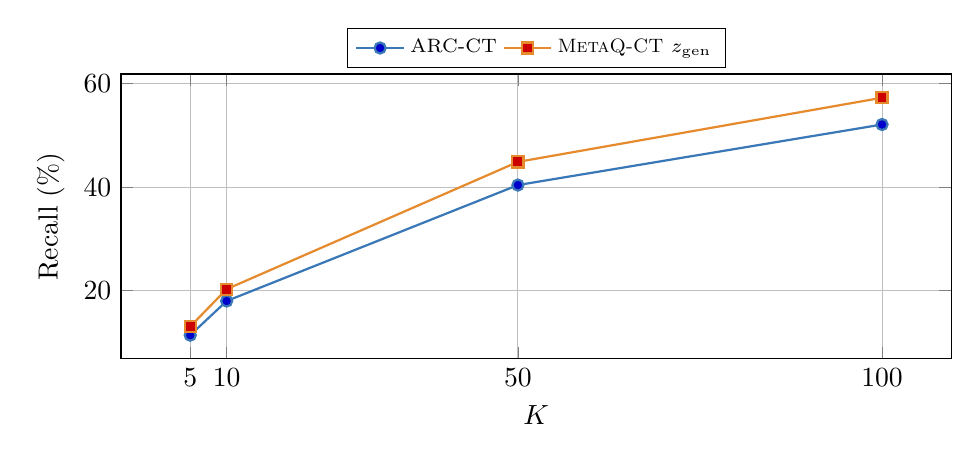
\begin{tikzpicture}
\begin{axis}[
  width=\columnwidth,height=5.2cm,
  xlabel={$K$},ylabel={Recall (\%)},
  xtick={5,10,50,100},grid=major,
  legend style={at={(0.5,1.02)},anchor=south,legend columns=2,font=\scriptsize}
]
\addplot+[mark=*,thick,color=ctblue] coordinates {(5,11.4)(10,18.0)(50,40.4)(100,52.1)};
\addplot+[mark=square*,thick,color=ctxorange] coordinates {(5,13.07)(10,20.29)(50,44.88)(100,57.27)};
\legend{ARC-CT,\ours{} $z_{\mathrm{gen}}$}
\end{axis}
\end{tikzpicture}
\caption{Canonical report-to-CT retrieval without retrieval-specific fitting.}
\label{fig:retrieval}
\end{figure}

\section{Discussion}
The adult result separates two things that a single AUROC number hides. The
architecture improves over its image-only branch by 0.48 points on the final
checkpoint, and an earlier three-seed campaign improved over a matched CT-only
control by 2.1 points. The intervention shows that only 0.27 points depend on
the indication being the patient's own.
The remainder is class-specific residual capacity that the conditioned bank
adds. Both facts are useful, and reporting only the first would be misleading.

This also explains where the design should pay off. Conditioning can only help
when the clinical text carries information the image does not. Adult CT-RATE
indications are often absent or generic, so there is little such information
to read. In a companion pediatric study using the same conditioning family, the
intervention gap is 3.0 to 4.4 points rather than 0.27. Pediatric
indications carry oncologic history, surgical context, transplant status, and
genetic diagnoses. The mechanism is the same in both cohorts. What differs is
how much the indication is worth.

Retrieval clarifies which component contributes what. The isolated general
bank retains a strong canonical embedding and achieves leading recall, while
post-hoc metadata mixing slightly degrades it. The conditioned pathway is
therefore a diagnosis-side addition and not a representation-side one.

\section{Limitations}
The adult evaluation uses one benchmark. CT-RATE is a single-institution
cohort, and its indication field is frequently empty, which directly limits
how much the conditioning can be shown to do. The supervised \texttt{ctx\_cls}
row and the Biltir paired rows are single selected checkpoints rather than
three-seed means, and they are labelled that way in every table. The newer
adult-only checkpoints still lack a complete true, blank, and shuffled
intervention, and their checkpoint-selection and reporting split is the same
3,002-study cache. They therefore cannot replace the independently selected
local benchmark estimate. The external RAD-ChestCT row that leads the table is a fitted
logistic readout and is not zero-shot. Report-generation numbers are
preliminary and carry no clinical claim. The benchmark comparison uses
published adult numbers for prior methods rather than local reruns, so
differences in preprocessing and threshold protocol cannot be fully excluded.

\section{Conclusion}
Conditioning pathology-specific query slots on the clinical indication, age,
and sex improves adult chest CT abnormality classification from 0.8733 to
0.8781 macro AUROC on the official CT-RATE validation split, and sets a new
prompt-based benchmark result. The causal contribution of the indication
itself is small on this cohort, at 0.27 AUROC points. We report the
gain and its cause separately. The same conditioning principle, applied where clinical
context is genuinely informative, produces a much larger and
intervention-confirmed effect.

\appendix
\section{Complete Per-Class Results}
Per-class prompt AUROC for the matched CT-only and conditioned models on the
official CT-RATE validation split is given in \Cref{tab:adultclass}.

\begin{table*}[t]
\centering
\caption{Adult CT-RATE per-class prompt AUROC, averaged over three seeds.}
\label{tab:adultclass}
\resizebox{\textwidth}{!}{%
\begin{tabular}{@{}lrrr@{\hspace{1.0cm}}lrrr@{}}
\toprule
Pathology & CT-only & C1 & $\Delta$ & Pathology & CT-only & C1 & $\Delta$ \\
\midrule
Medical material & .9159 & .9447 & +.0287 & Lung nodule & .7270 & .7383 & +.0113 \\
Arterial wall calcification & .9336 & .9421 & +.0085 & Lung opacity & .8680 & .8844 & +.0164 \\
Cardiomegaly & .9343 & .9364 & +.0021 & Pulmonary fibrotic sequela & .7020 & .7463 & +.0443 \\
Pericardial effusion & .8957 & .9040 & +.0083 & Pleural effusion & .9768 & .9725 & -.0042 \\
Coronary wall calcification & .9273 & .9381 & +.0109 & Mosaic attenuation & .8163 & .8954 & +.0790 \\
Hiatal hernia & .8159 & .8209 & +.0050 & Peribronchial thickening & .8148 & .8261 & +.0113 \\
Lymphadenopathy & .7786 & .7923 & +.0136 & Consolidation & .9285 & .9334 & +.0049 \\
Emphysema & .8113 & .8251 & +.0138 & Bronchiectasis & .7995 & .8242 & +.0247 \\
Atelectasis & .7967 & .8103 & +.0136 & Interlobular septal thickening & .8120 & .8951 & +.0831 \\
\multicolumn{4}{c}{} & \textbf{Macro mean} & \textbf{.8475} & \textbf{.8683} & \textbf{+.0209} \\
\bottomrule
\end{tabular}}
\end{table*}

\section{Auxiliary Supervised Readout}
The best separate \texttt{ctx\_cls} checkpoint reaches 0.88386 macro AUROC on
all 3,002 CT-RATE validation studies and 0.88484 on the 1,464-study
indication-present subset. Full-split per-class values are listed in
\Cref{tab:ctxclsclass}. This appendix is deliberately separate from the
prompt-based primary result. A single-checkpoint training-cohort comparison
also favors using the full available CT-RATE cache: 0.88386 versus 0.86937 on
the full validation cache (\Cref{tab:ctxclsdata}). These values share the
Biltir model-selection caveat described above.

\begin{table}[t]
\centering
\caption{Exploratory \texttt{ctx\_cls} training-data comparison.}
\label{tab:ctxclsdata}
\resizebox{\columnwidth}{!}{%
\begin{tabular}{@{}lrr@{}}
\toprule
Training cohort & Full $N=3{,}002$ & Ind.-present $N=1{,}464$ \\
\midrule
Indication-present only & 0.86937 & 0.87585 \\
Full CT-RATE cache & \best{0.88386} & \best{0.88484} \\
\bottomrule
\end{tabular}}
\end{table}

\begin{table*}[t]
\centering
\caption{Per-class AUROC of the supervised \texttt{ctx\_cls} checkpoint.}
\label{tab:ctxclsclass}
\begin{tabular}{@{}lrr@{\hspace{1.4cm}}lrr@{}}
\toprule
Pathology & Full & Ind.-present & Pathology & Full & Ind.-present \\
\midrule
Medical material & .9443 & .9390 & Lung nodule & .8052 & .8037 \\
Arterial wall calcification & .9426 & .9423 & Lung opacity & .8909 & .9004 \\
Cardiomegaly & .9442 & .9374 & Pulmonary fibrotic sequela & .7742 & .7831 \\
Pericardial effusion & .9287 & .9398 & Pleural effusion & .9767 & .9719 \\
Coronary wall calcification & .9460 & .9354 & Mosaic attenuation & .9135 & .9149 \\
Hiatal hernia & .8519 & .8707 & Peribronchial thickening & .8316 & .8165 \\
Lymphadenopathy & .7998 & .7867 & Consolidation & .9263 & .9338 \\
Emphysema & .8420 & .8310 & Bronchiectasis & .8553 & .8518 \\
Atelectasis & .8359 & .8540 & Interlobular septal thickening & .9005 & .9147 \\
\midrule
\multicolumn{3}{c}{} & \textbf{Macro mean} & \textbf{.88386} & \textbf{.88484} \\
\bottomrule
\end{tabular}
\end{table*}

\bibliographystyle{plain}
\bibliography{references}

\end{document}
